% =============================================
% CAPÍTULO 3 - ANÁLISE DE VIABILIDADE
% =============================================
\chapter{ANÁLISE DE VIABILIDADE}

Para que uma solução tecnológica apresente potencial real de implantação, não basta considerar apenas seu desenvolvimento técnico, sendo igualmente necessário avaliar sua aceitação pelo público, sua viabilidade operacional e suas possibilidades de monetização. No caso deste projeto, a análise de viabilidade busca verificar se uma solução de assistência financeira inteligente, operada por meio do WhatsApp, é relevante para o público-alvo, economicamente sustentável e tecnicamente executável. Essa avaliação torna-se especialmente importante por se tratar de um produto que depende tanto da interação em um canal de mensageria empresarial quanto da integração com dados compartilhados no ecossistema de \textit{Open Finance}, o qual funciona sob consentimento do usuário e em ambiente seguro.

\section{Análise de demanda}

De acordo com Iunes (1995), a demanda pode ser definida como a relação direta entre a quantidade de determinado bem ou serviço que os consumidores desejam obter e o seu poder aquisitivo em um dado período. Portanto, torna-se essencial realizar uma análise de demanda assertiva e objetiva, buscando compreender quais fenômenos e variáveis influenciam a procura por um produto ou serviço dentro do mercado consumidor e, com isso, estabelecer estratégias adequadas ao cenário encontrado.

A fim de possibilitar essa análise e obter dados que garantam a viabilidade de desenvolvimento do projeto proposto, foi aplicado como metodologia de levantamento de dados um questionário quantitativo, cujos principais objetivos foram verificar se os potenciais usuários enfrentam dificuldades concretas na gestão financeira pessoal, mensurar o interesse por um assistente conversacional baseado em inteligência artificial integrado ao WhatsApp e avaliar a familiaridade com o ecossistema de \textit{Open Finance}. O questionário, cujas questões são detalhadas no Apêndice A, foi respondido por 42 participantes entre 06 e 20 de abril de 2026, por meio da ferramenta Google Forms. O perfil predominante dos respondentes foi de adultos entre 25 e 44 anos, com ensino superior completo ou incompleto, distribuídos entre os sexos feminino (22) e masculino (19). O detalhamento completo das respostas encontra-se na Tabela \ref{tab:questionario}, no Apêndice B.

Inicialmente, foi possível constatar que o WhatsApp já faz parte do cotidiano de praticamente todos os respondentes, com 41 dos 42 participantes (97,6\%) afirmando utilizá-lo diariamente, o que indica uma alta aderência ao canal escolhido para a solução. Em relação aos hábitos financeiros, o gráfico da Figura \ref{fig:pq_frequencia} demonstra que a consulta ao saldo bancário é frequente: 22 respondentes (52,4\%) o fazem diariamente e 11 (26,2\%) de duas a três vezes por semana, evidenciando um envolvimento ativo com a própria vida financeira.

\begin{figure}[H]
    \centering
    \caption{Frequência de consulta ao saldo bancário pelos respondentes}
    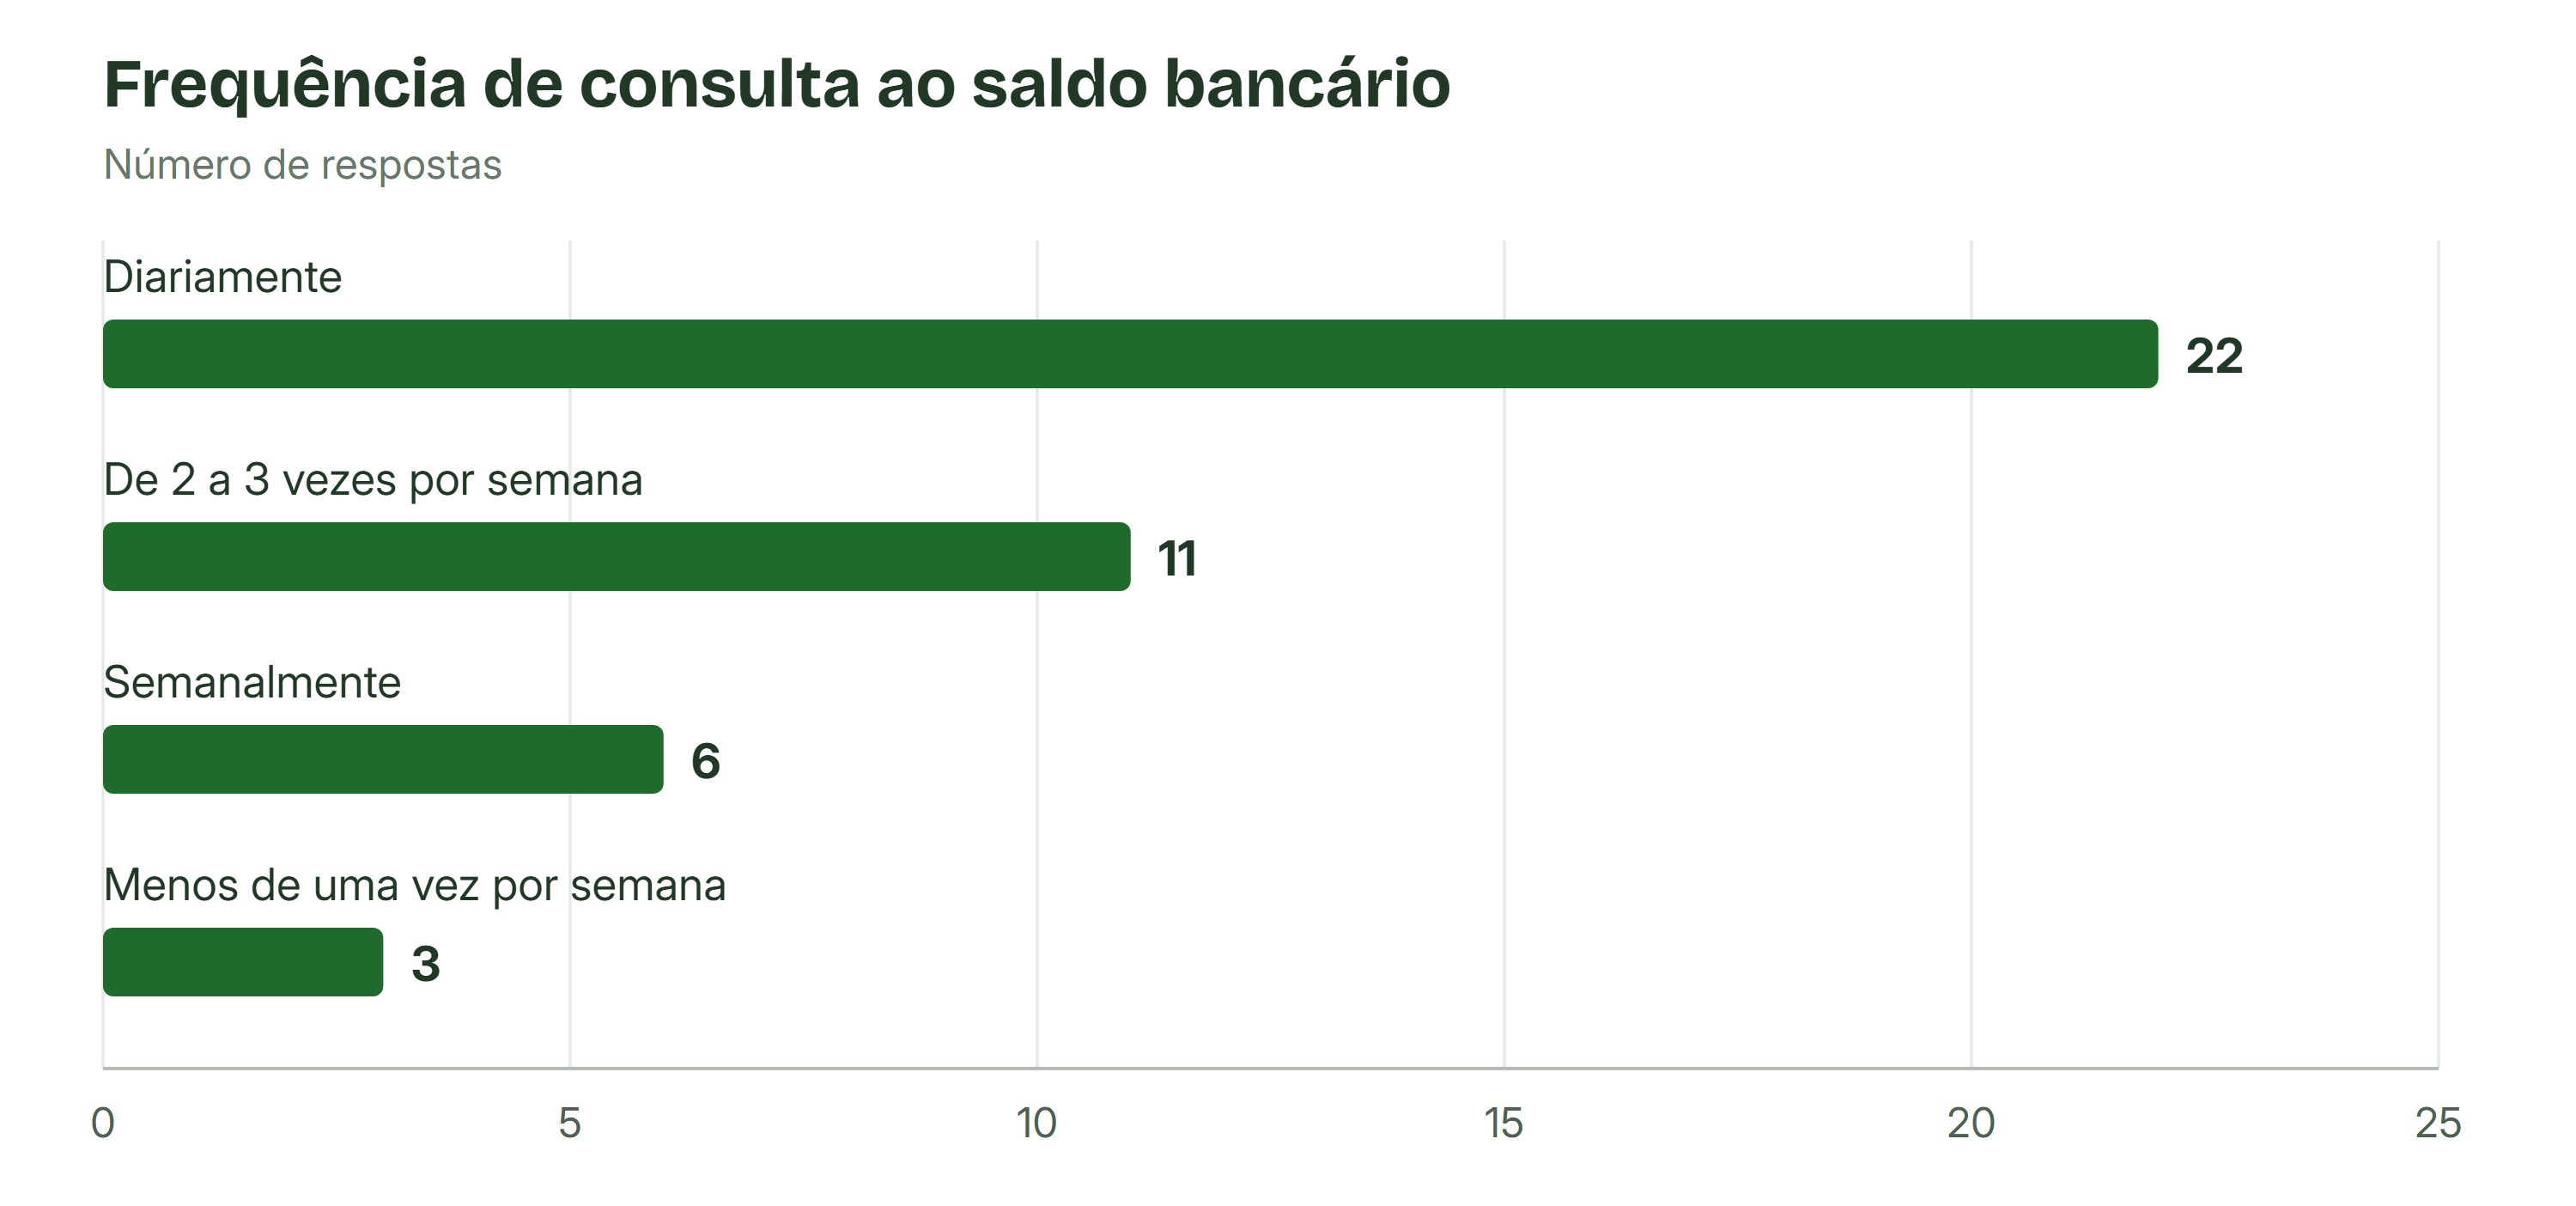
\includegraphics[width=0.8\textwidth]{images/pesquisa/frequenciaconsulta.png}
    \label{fig:pq_frequencia}
    \fontetabela{\textbf{Fonte:} Elaborado pelos autores (2026).}
\end{figure}

O gráfico da Figura \ref{fig:pq_contas} revelou que 17 respondentes (40,5\%) possuem duas contas bancárias ativas e 12 (28,6\%) possuem três, totalizando mais de 69\% dos participantes com múltiplas contas. Esse dado reforça a necessidade de uma solução que consolide e centralize informações financeiras dispersas entre diferentes instituições, exatamente o que o ecossistema de \textit{Open Finance} viabiliza.

\begin{figure}[H]
    \centering
    \caption{Número de contas bancárias ativas dos respondentes}
    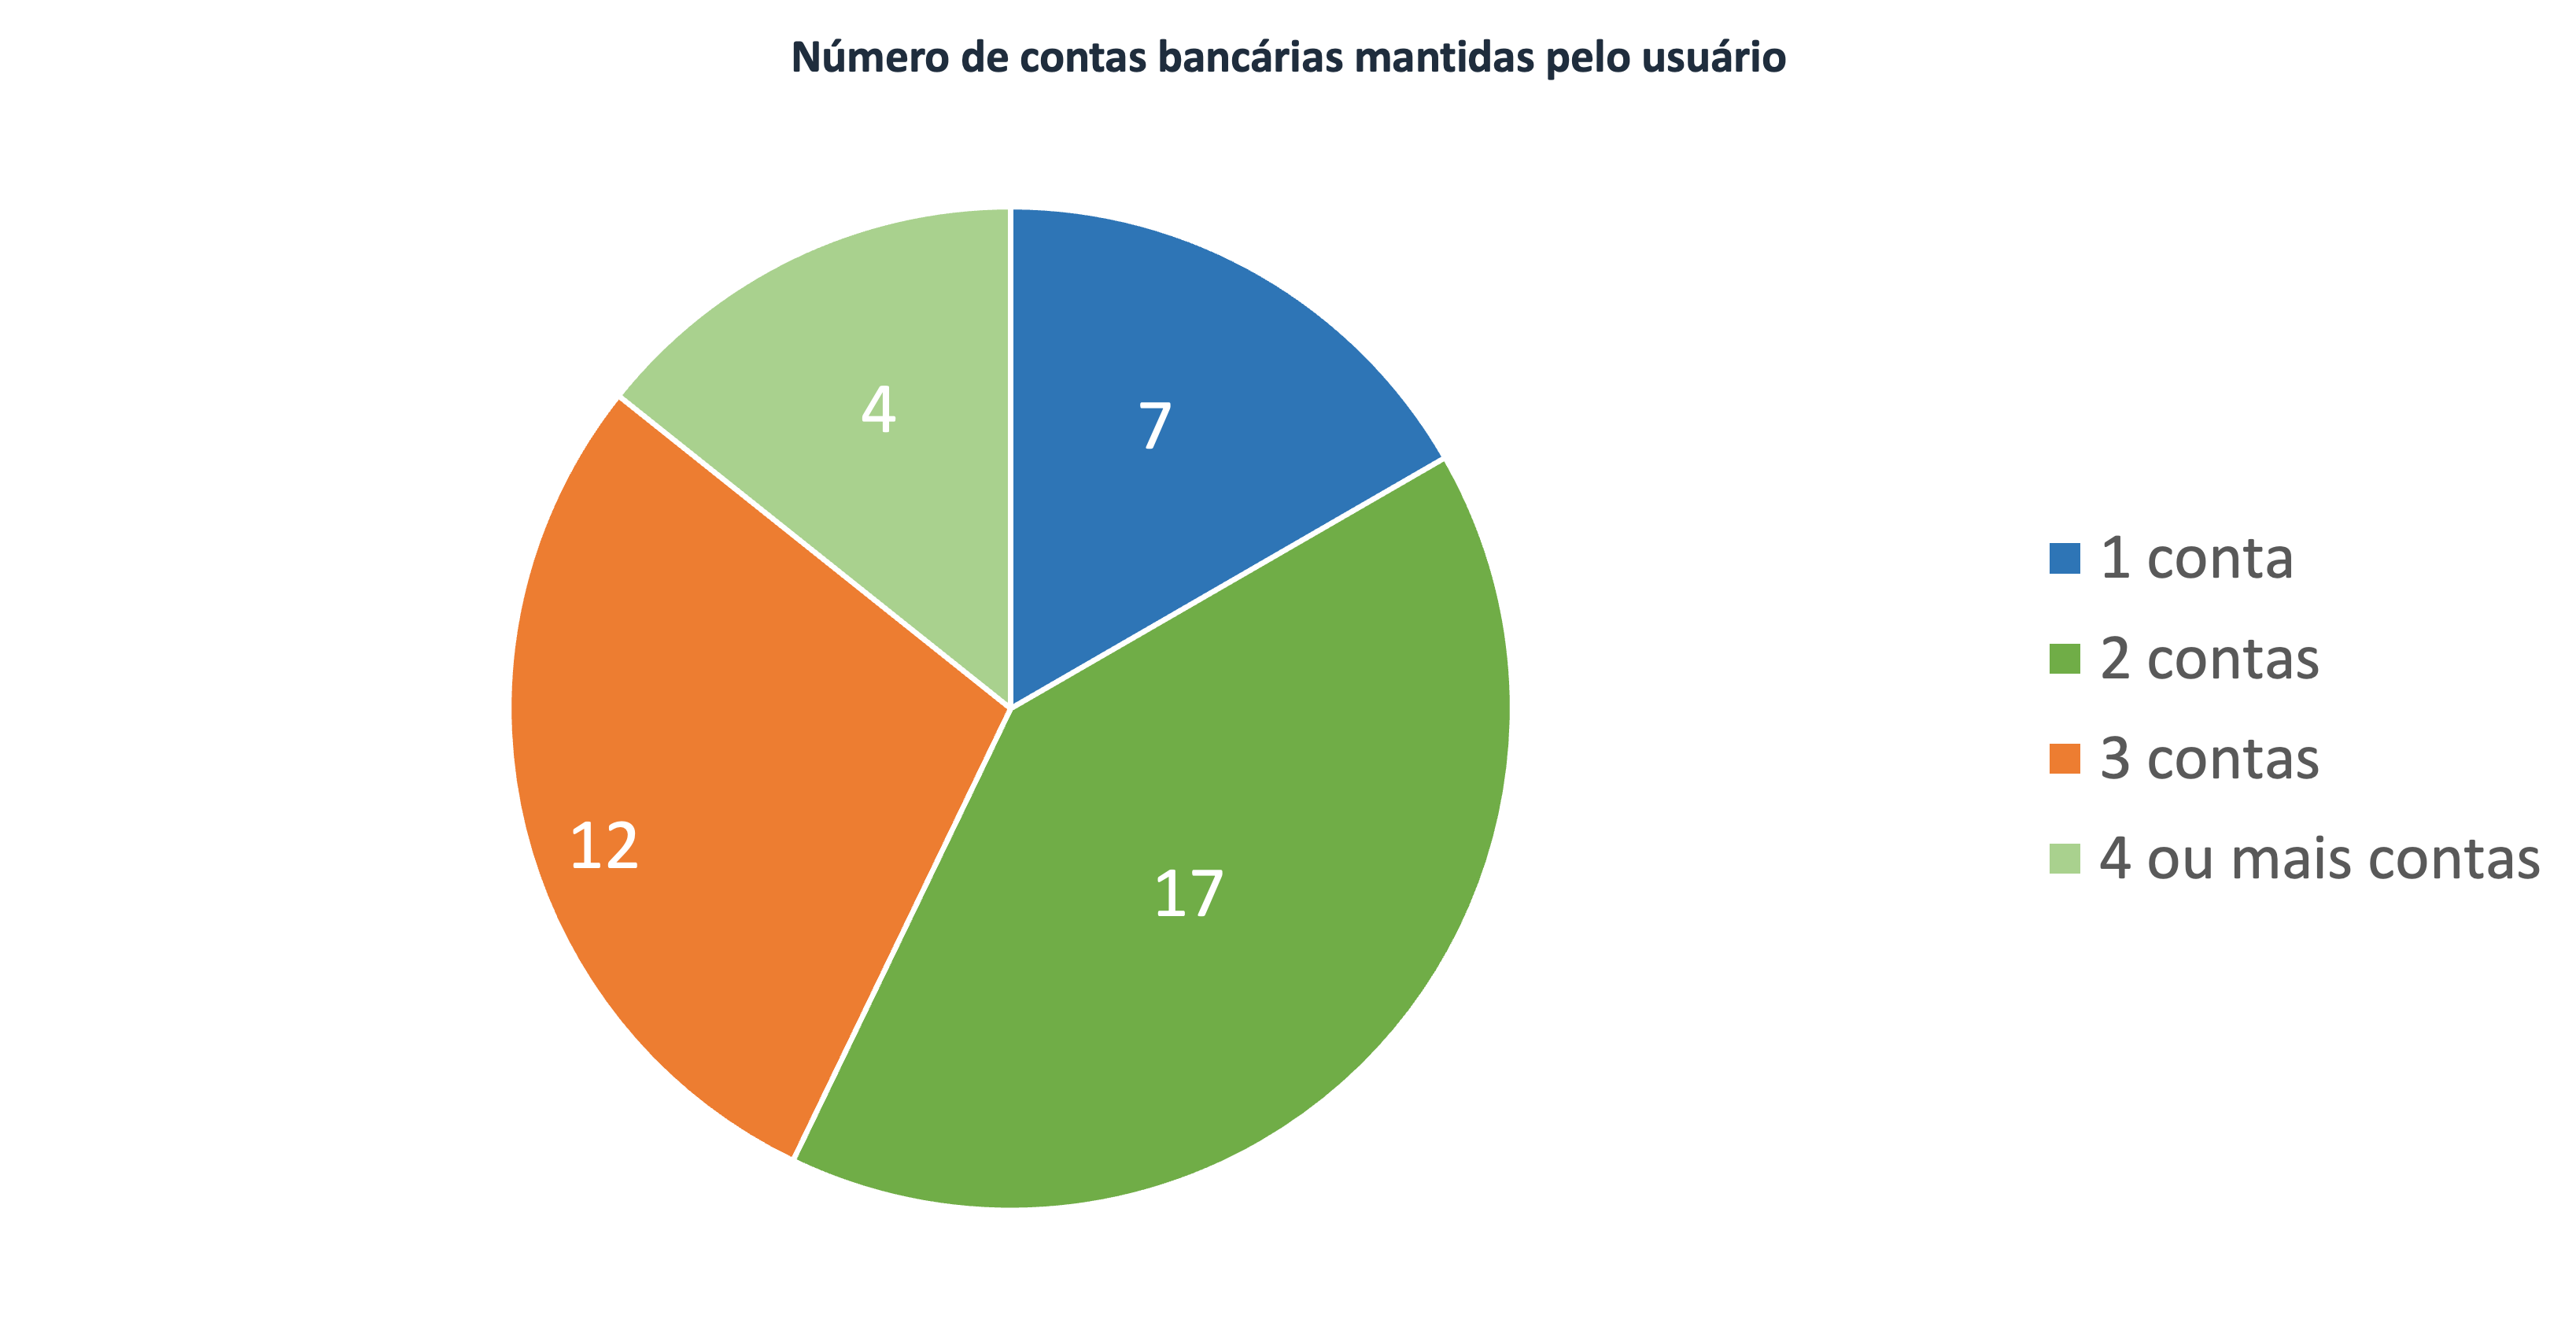
\includegraphics[width=0.8\textwidth]{images/pesquisa/numerocontas.png}
    \label{fig:pq_contas}
    \fontetabela{\textbf{Fonte:} Elaborado pelos autores (2026).}
\end{figure}

O gráfico da Figura \ref{fig:pq_openfinance} expôs ainda um expressivo desconhecimento do \textit{Open Finance}: 21 respondentes (50\%) declararam não conhecer o ecossistema, e apenas 4 (9,5\%) já compartilharam dados entre instituições. Esse resultado indica que existe uma oportunidade de educação e introdução ao tema dentro da própria plataforma, tornando-a um veículo de adoção gradual do \textit{Open Finance} junto ao usuário final.

\begin{figure}[H]
    \centering
    \caption{Familiaridade dos respondentes com o Open Finance}
    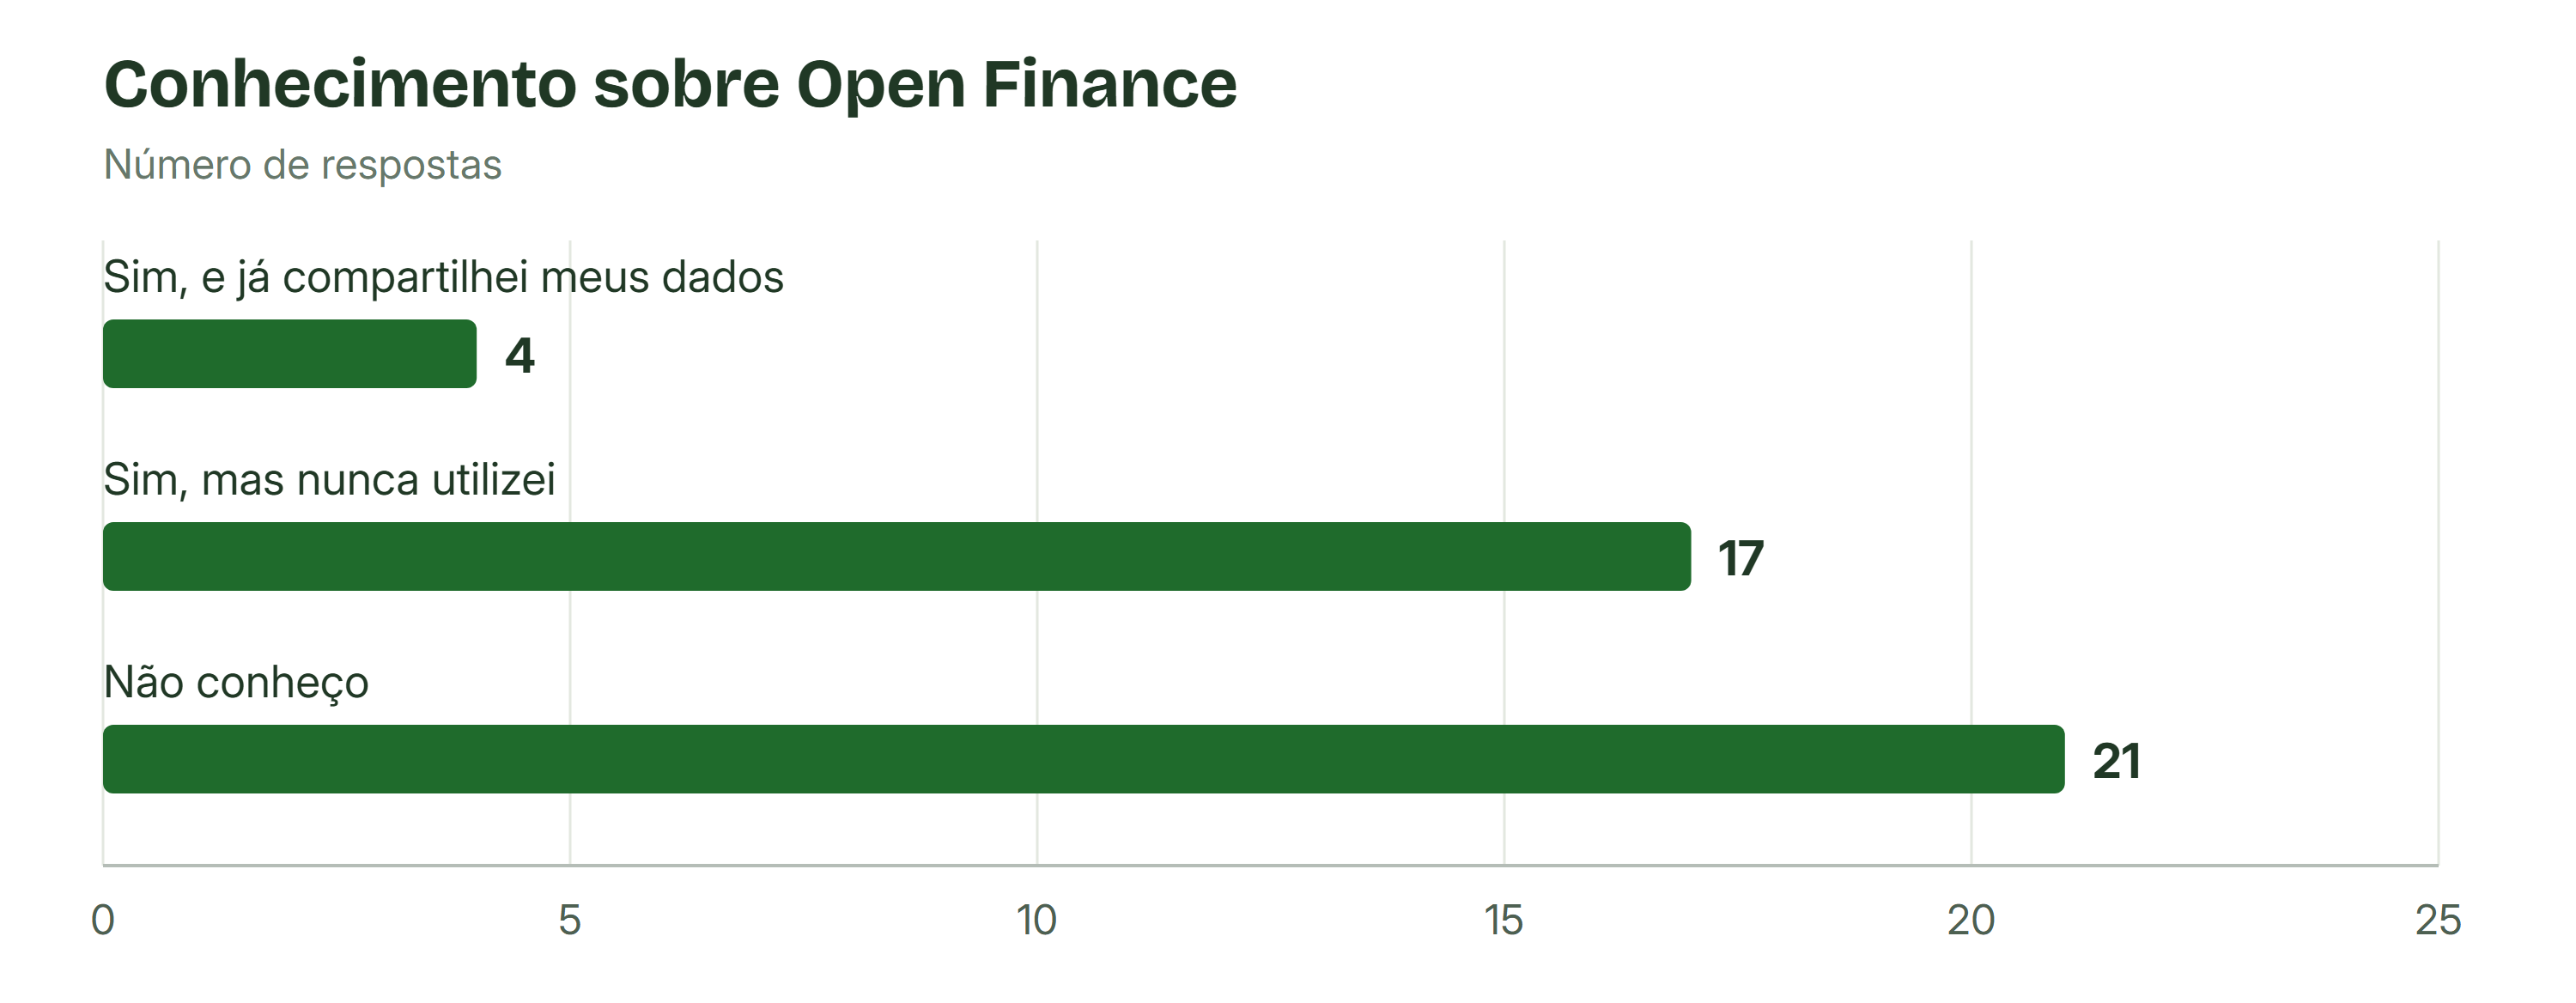
\includegraphics[width=0.8\textwidth]{images/pesquisa/conhecimentoopenfinance.png}
    \label{fig:pq_openfinance}
    \fontetabela{\textbf{Fonte:} Elaborado pelos autores (2026).}
\end{figure}

Em seguida, o gráfico da Figura \ref{fig:pq_funcionalidades} demonstrou elevado interesse nas funcionalidades propostas: resumo automático de gastos (32 respondentes), alerta de vencimento de contas (29), previsão de saldo (26), recomendações personalizadas (23) e detecção de gastos atípicos (21). A demanda por essas funções confirma que o problema identificado é percebido concretamente pelo público-alvo e que a solução proposta apresenta aderência às necessidades reais dos usuários.

\begin{figure}[H]
    \centering
    \caption{Funcionalidades de maior interesse para os respondentes}
    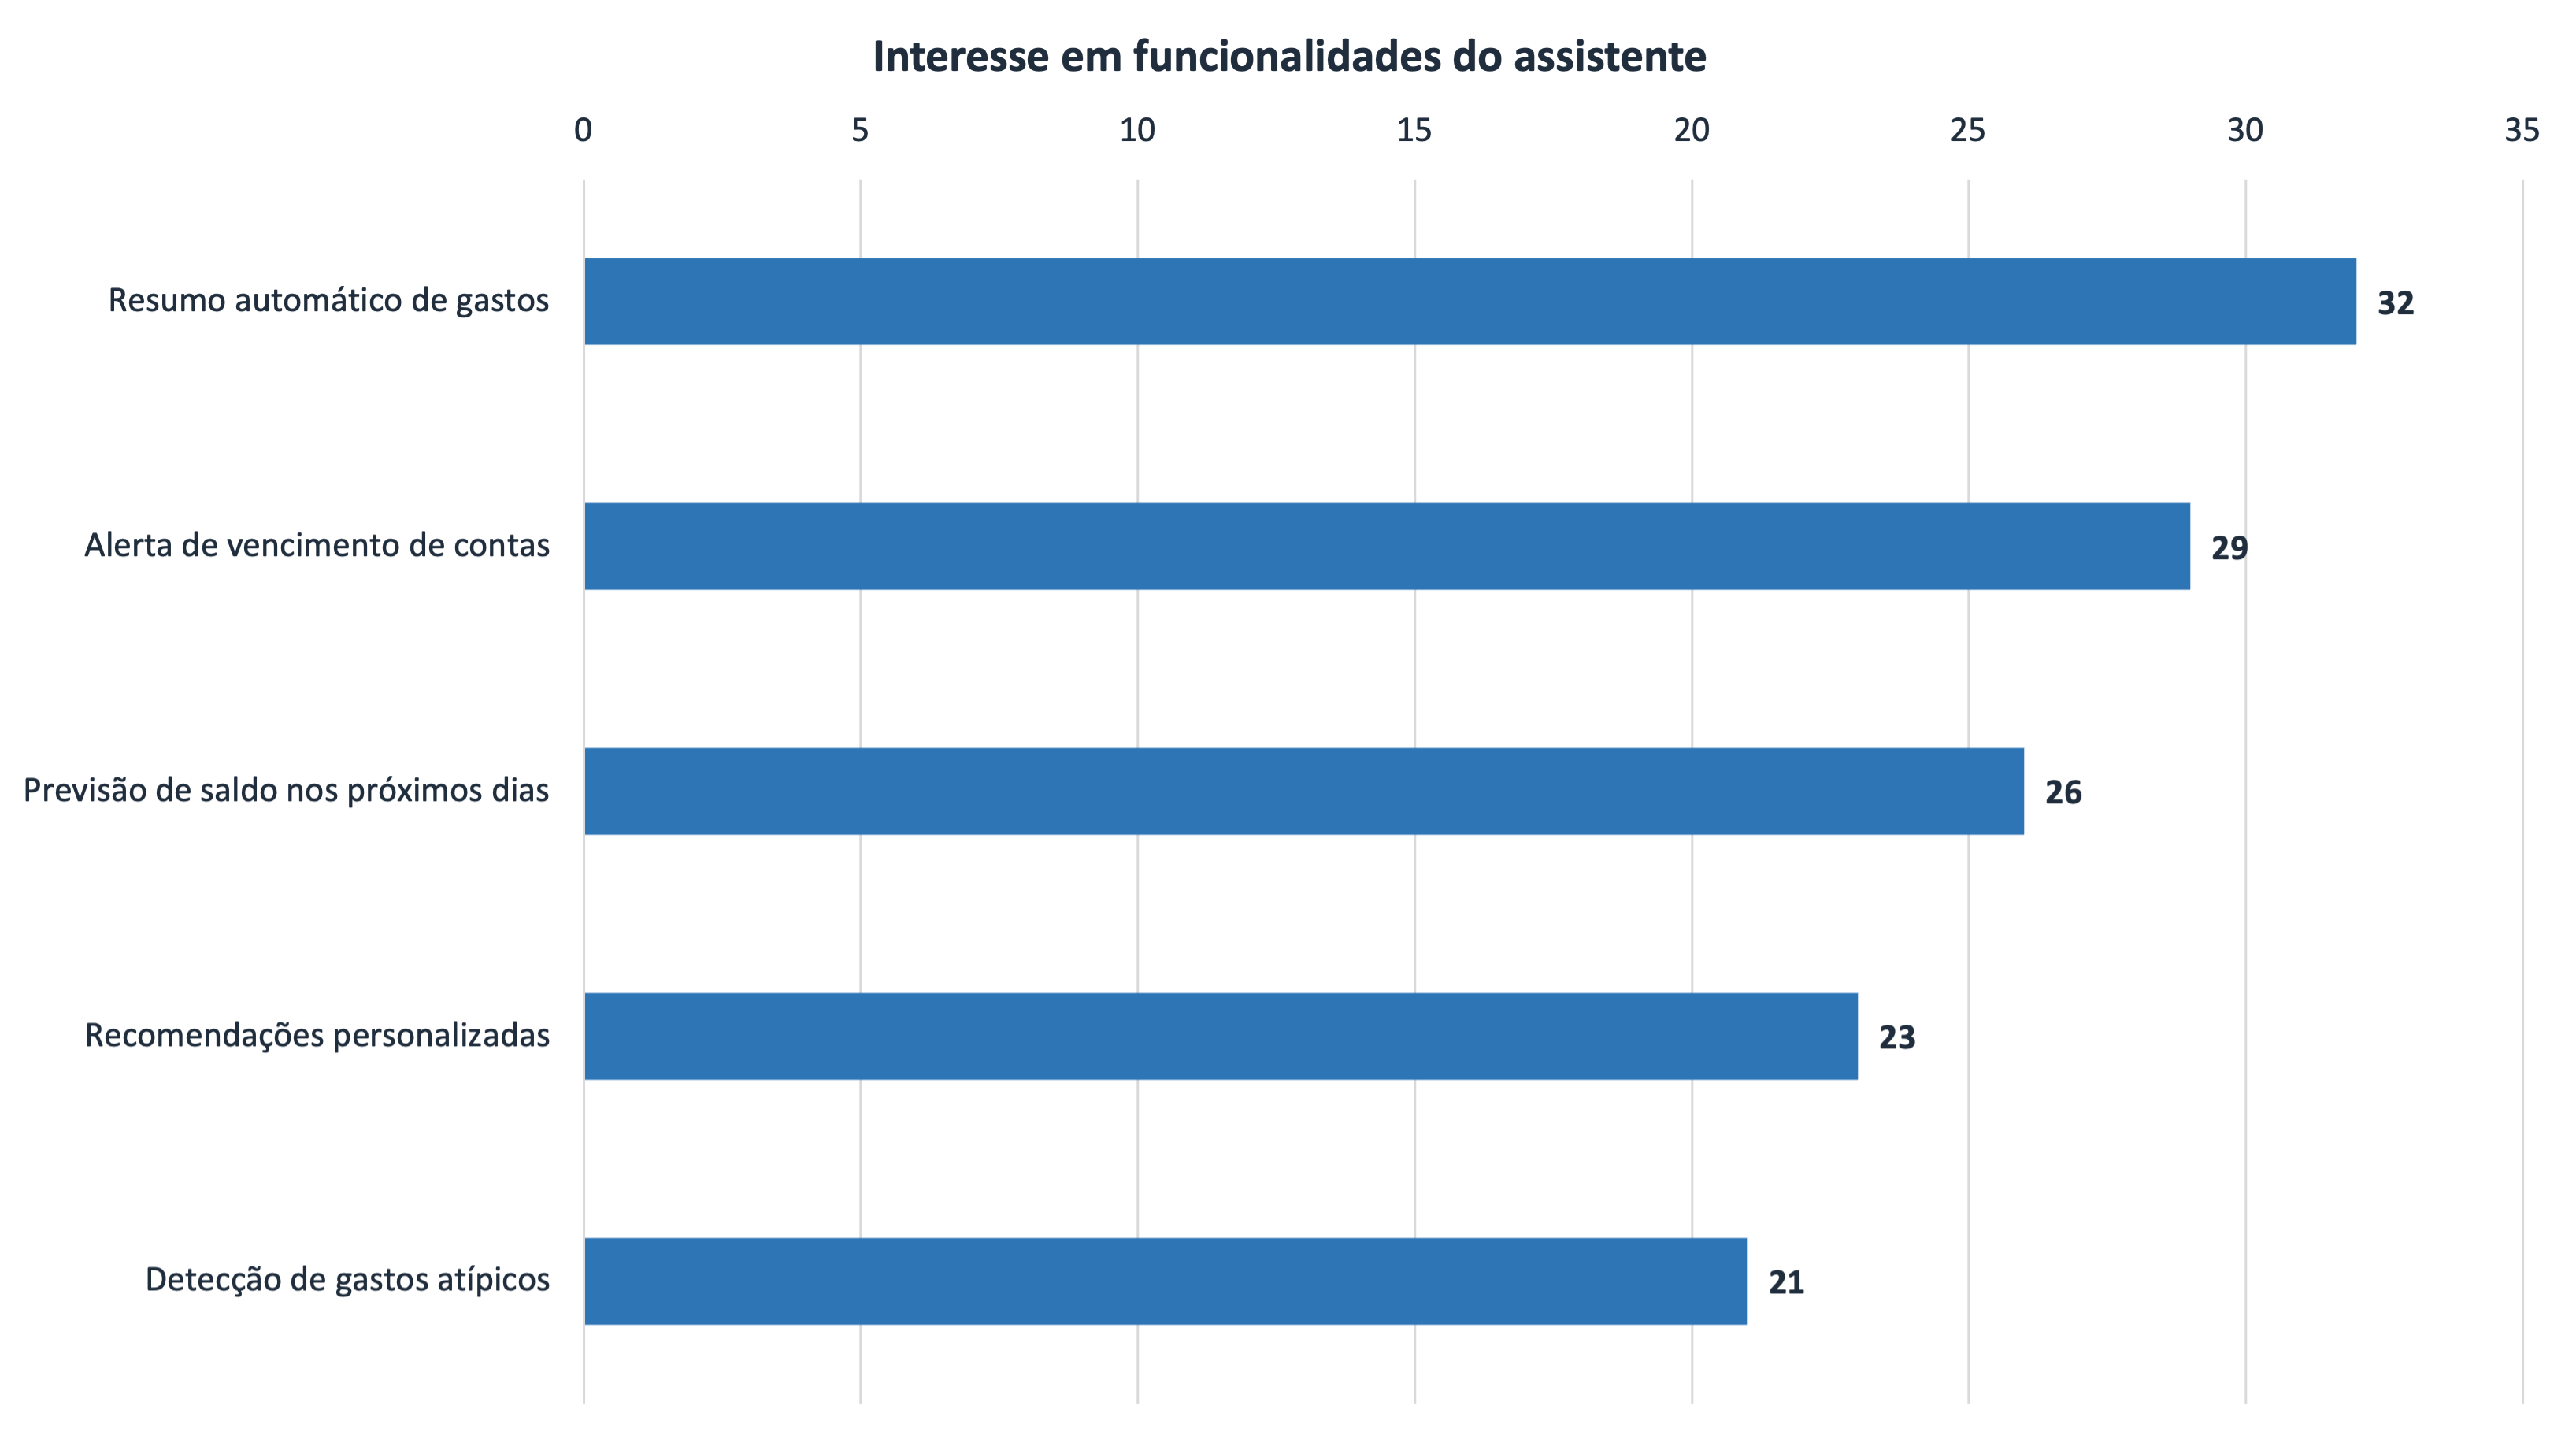
\includegraphics[width=0.8\textwidth]{images/pesquisa/interessefuncionalidade.png}
    \label{fig:pq_funcionalidades}
    \fontetabela{\textbf{Fonte:} Elaborado pelos autores (2026).}
\end{figure}

Por meio do gráfico da Figura \ref{fig:pq_confianca}, foi possível verificar o nível de confiança dos respondentes em um assistente conversacional baseado em inteligência artificial para tratar de dados financeiros: as notas 4 e 5 somadas representam 47,6\% das respostas (20 participantes), enquanto apenas 26,2\% atribuíram notas 1 ou 2. O resultado indica que a maioria dos potenciais usuários apresenta predisposição favorável ao uso da tecnologia no contexto financeiro, embora ainda haja espaço para construir confiança por meio de transparência e segurança.

\begin{figure}[H]
    \centering
    \caption{Nível de confiança dos respondentes em assistente conversacional com IA}
    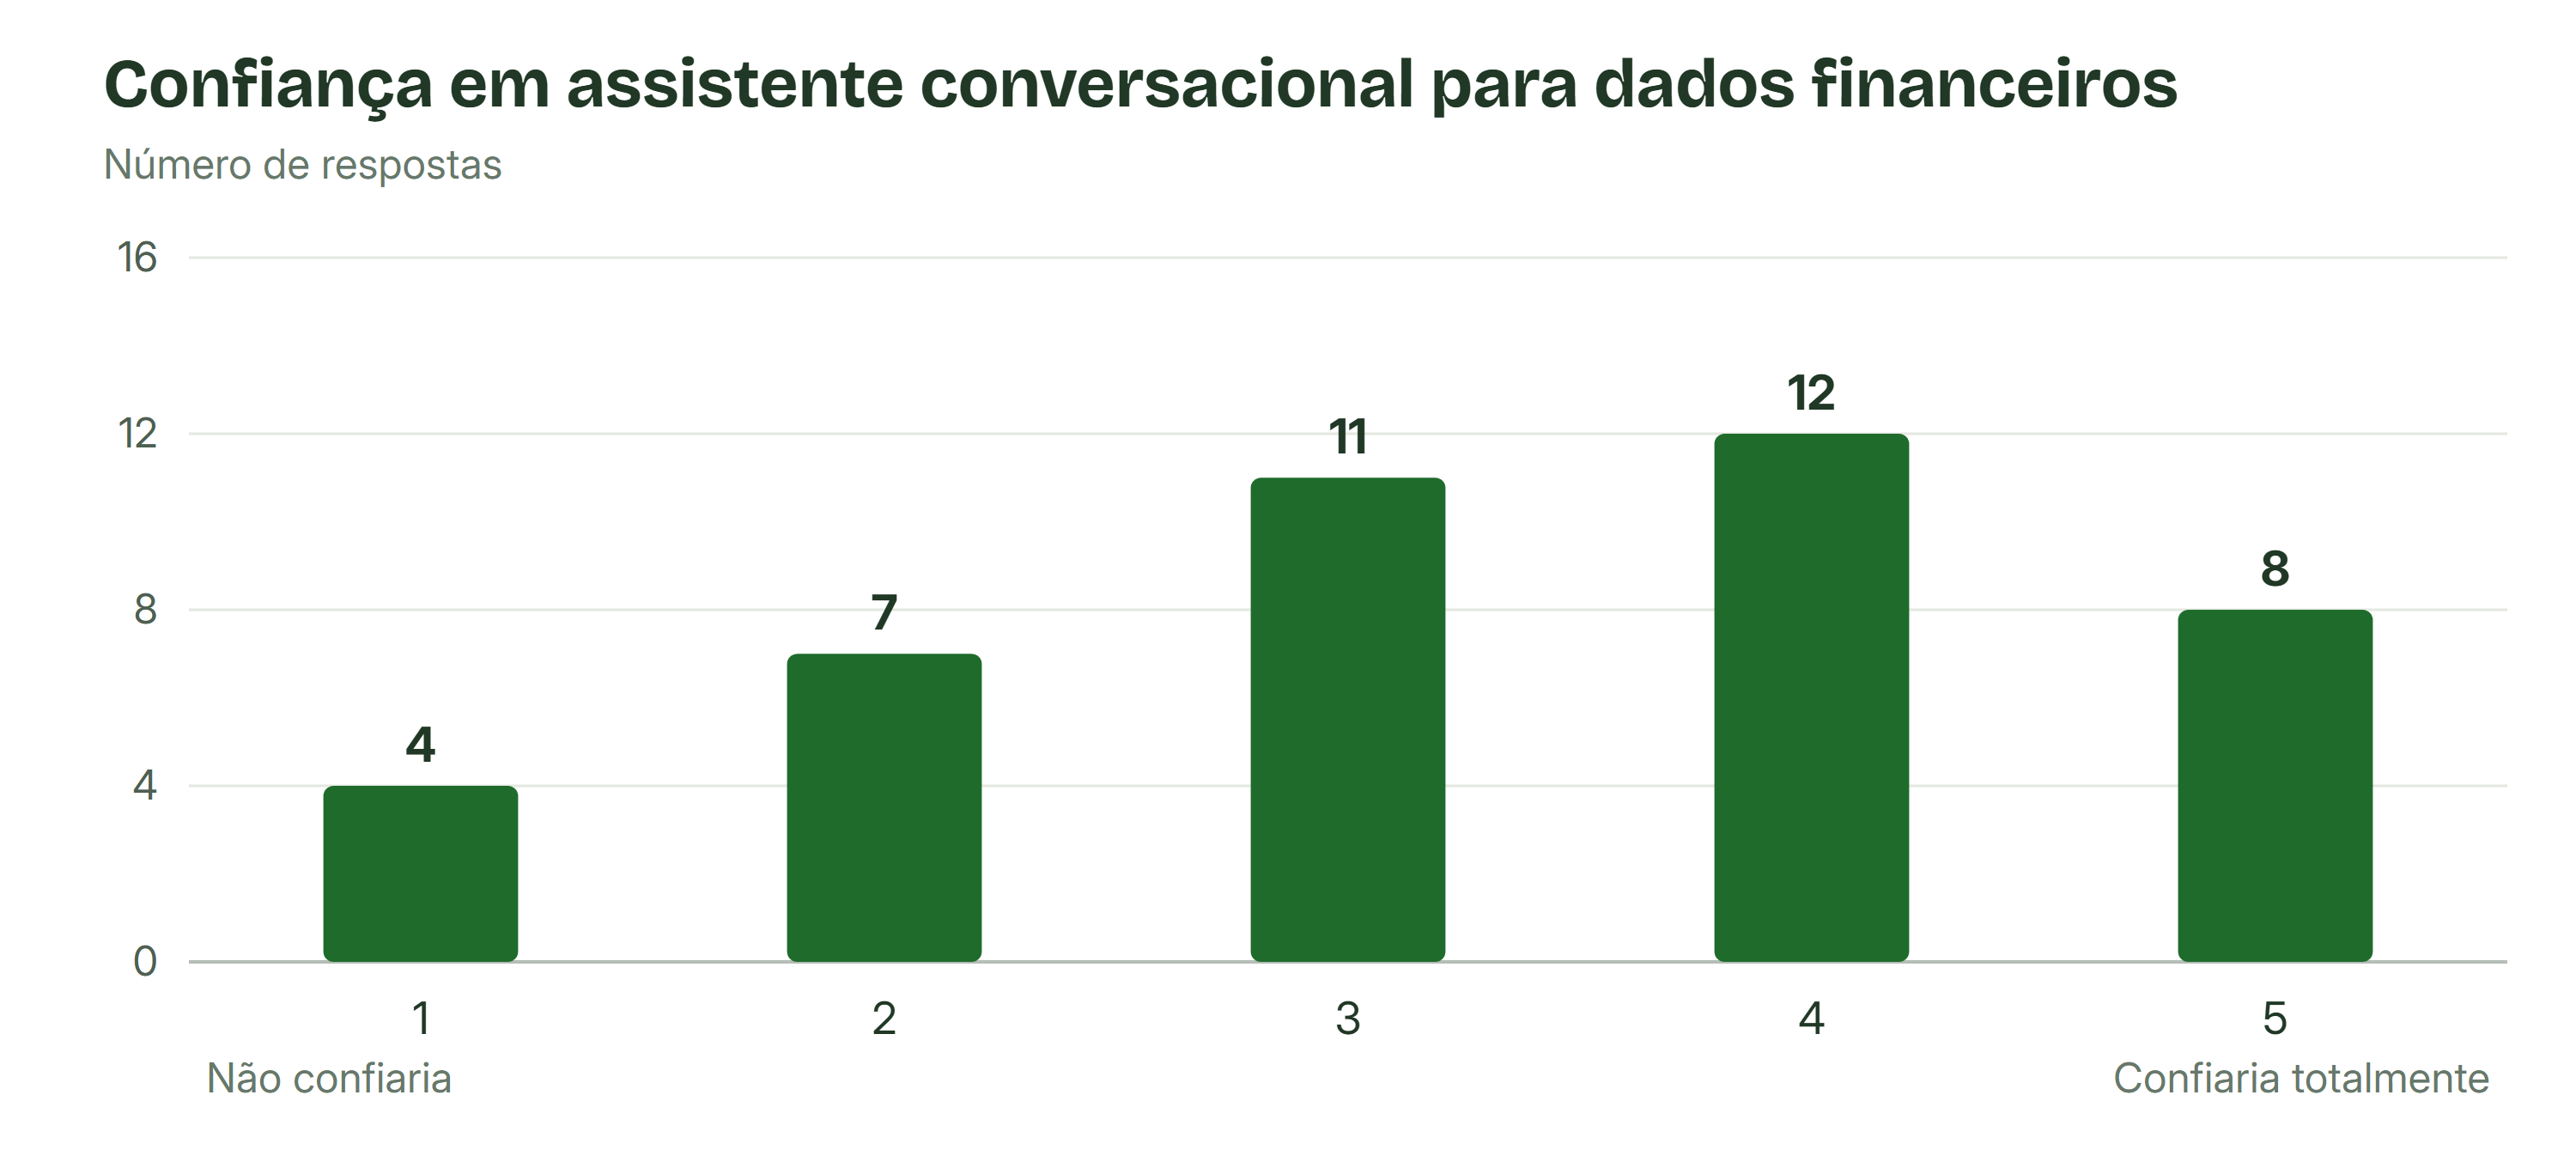
\includegraphics[width=0.8\textwidth]{images/pesquisa/confianca.png}
    \label{fig:pq_confianca}
    \fontetabela{\textbf{Fonte:} Elaborado pelos autores (2026).}
\end{figure}

O gráfico da Figura \ref{fig:pq_privacidade} indicou alto nível de preocupação com a privacidade dos dados financeiros: 15 respondentes (35,7\%) atribuíram nota máxima e 14 (33,3\%) nota 4, totalizando 69\% com preocupação elevada. Esse resultado reforça a necessidade de que a solução adote mecanismos robustos de proteção e transparência no tratamento dos dados, em conformidade com a LGPD.

\begin{figure}[H]
    \centering
    \caption{Nível de preocupação dos respondentes com a privacidade de dados financeiros}
    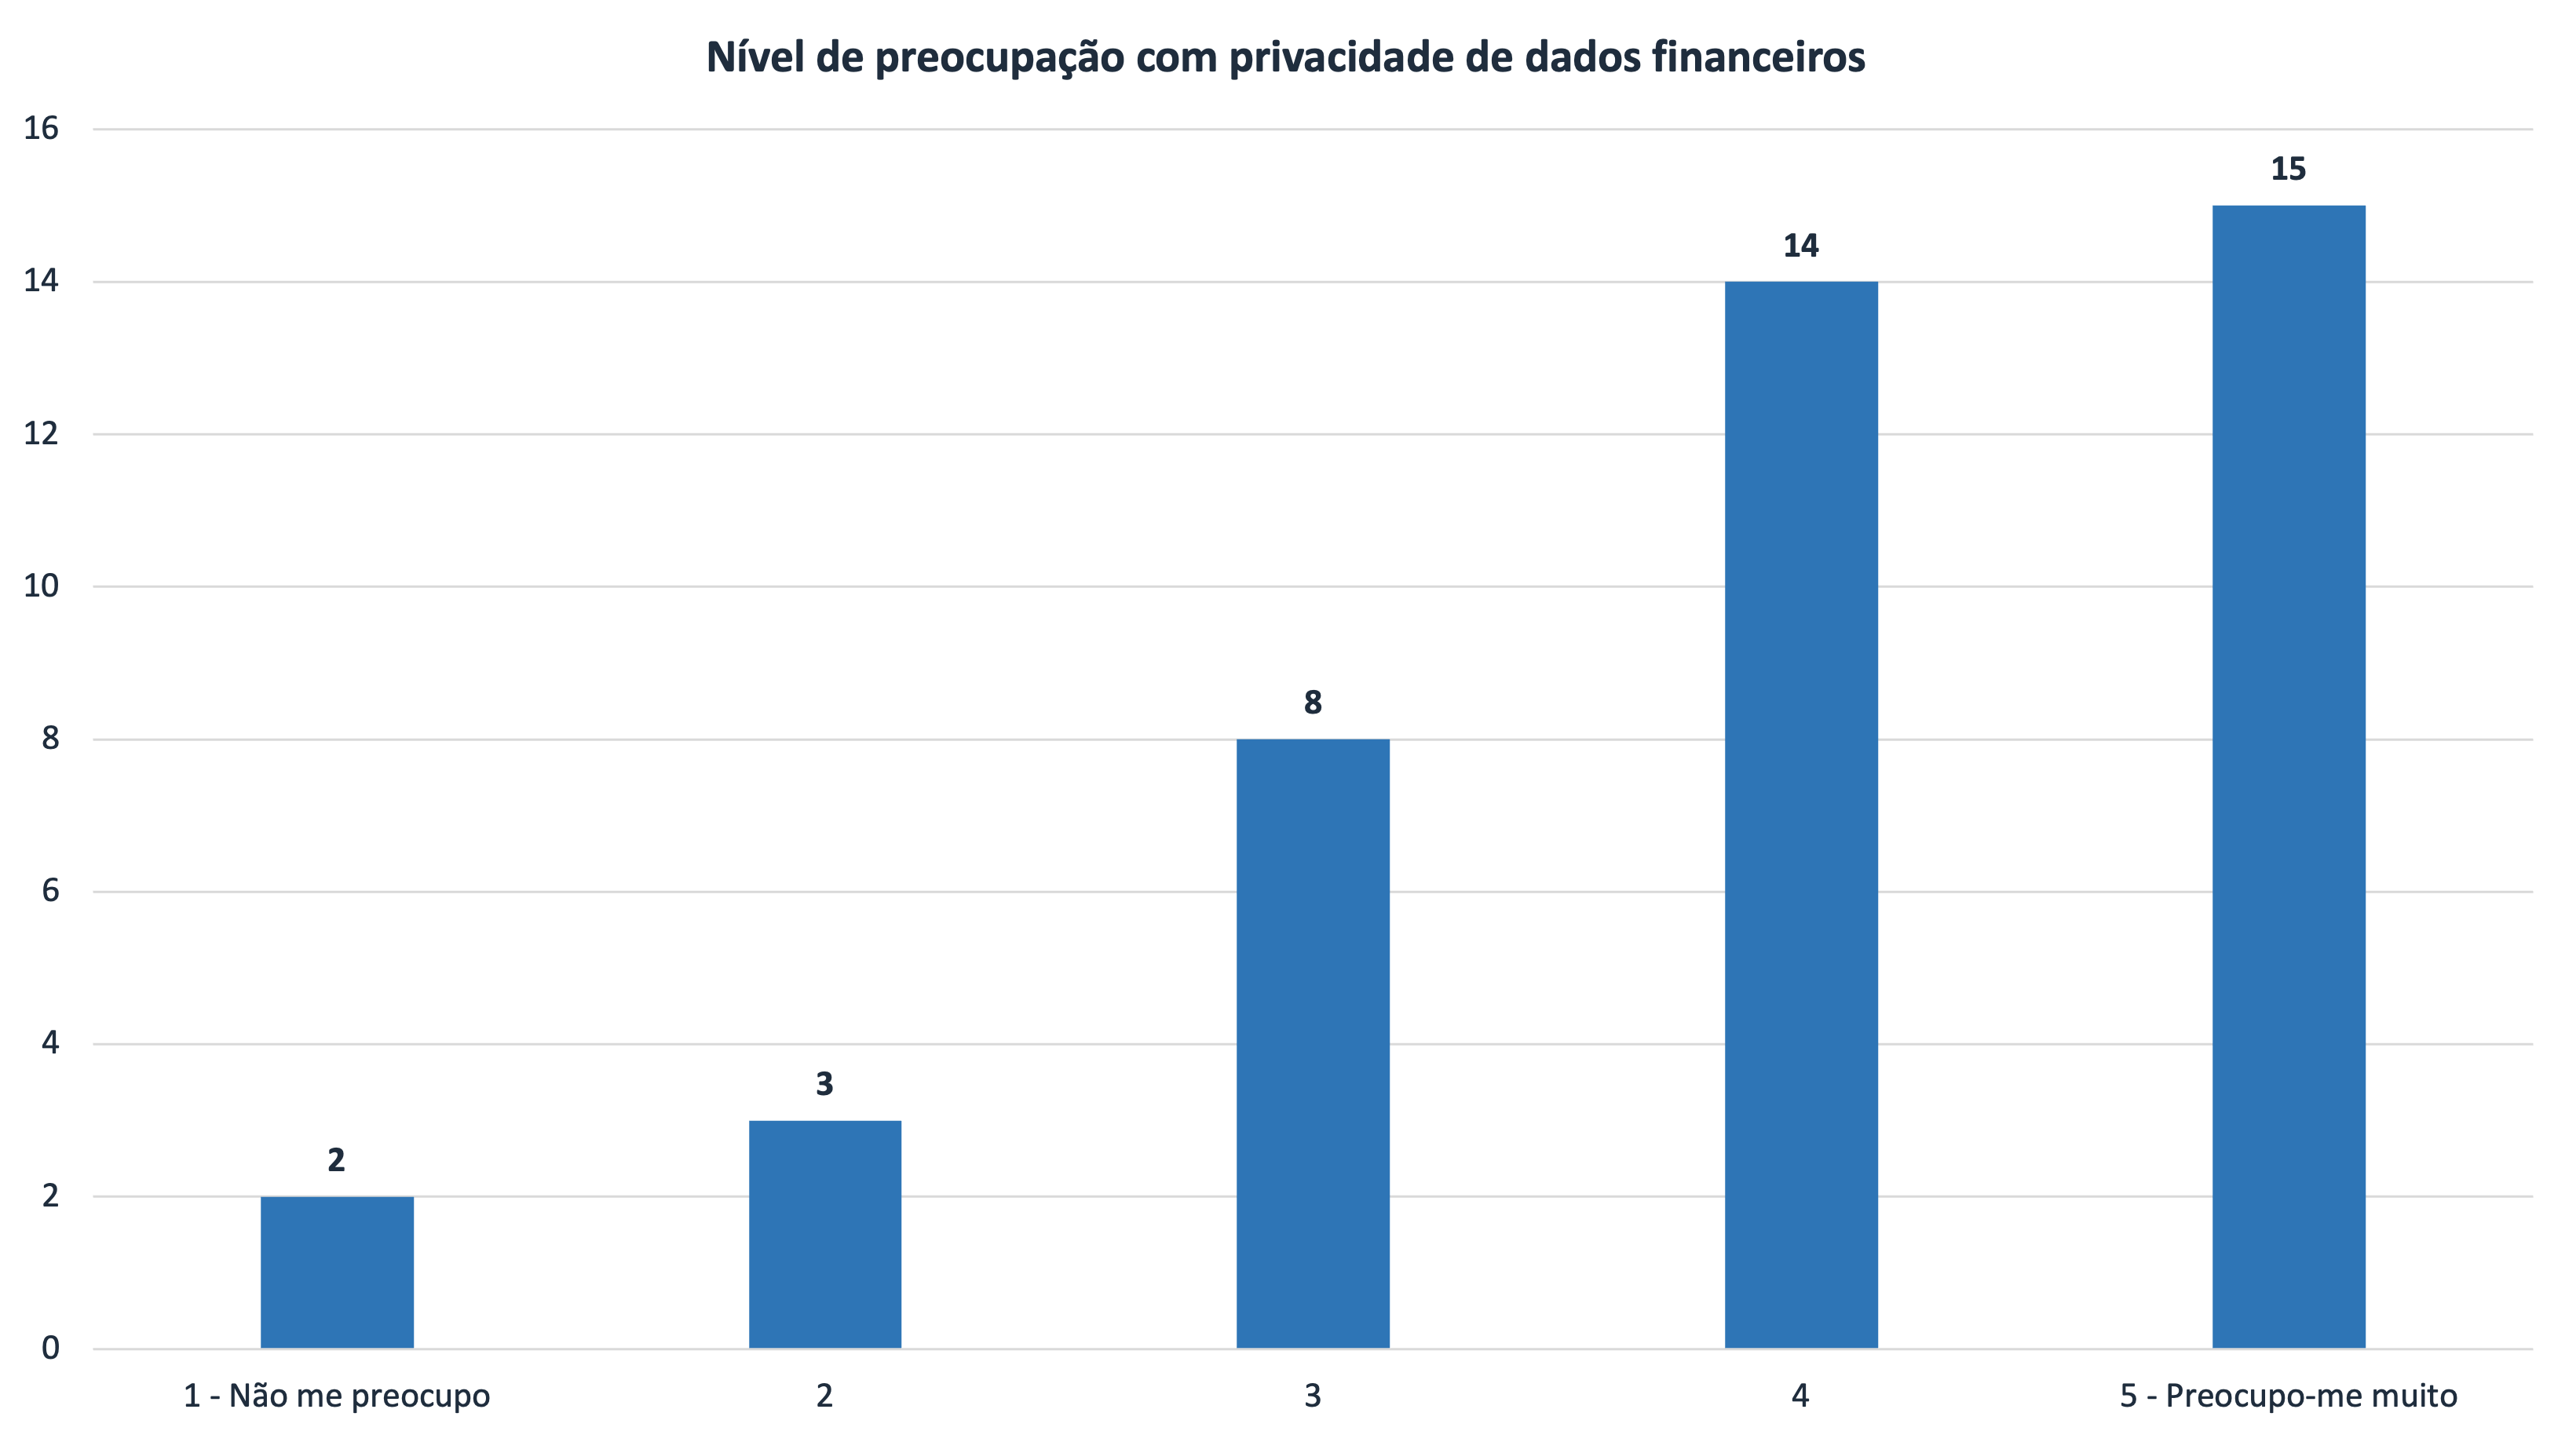
\includegraphics[width=0.8\textwidth]{images/pesquisa/nivelpreocupacao.png}
    \label{fig:pq_privacidade}
    \fontetabela{\textbf{Fonte:} Elaborado pelos autores (2026).}
\end{figure}

Finalmente, o gráfico da Figura \ref{fig:pq_pagamento} indicou que a maioria dos participantes demonstrou disposição para pagar pelo serviço: apenas 7 respondentes (16,7\%) afirmaram que não pagariam, enquanto 15 (35,7\%) aceitariam pagar entre R\$~11,00 e R\$~20,00 mensais e 12 (28,6\%) pagariam até R\$~10,00. Esses dados sustentam a viabilidade do modelo de monetização \textit{freemium} descrito na Seção \ref{sec:preco}, sugerindo que há margem para conversão de usuários gratuitos em assinantes pagos.

\begin{figure}[H]
    \centering
    \caption{Disposição dos respondentes para pagar por plano premium}
    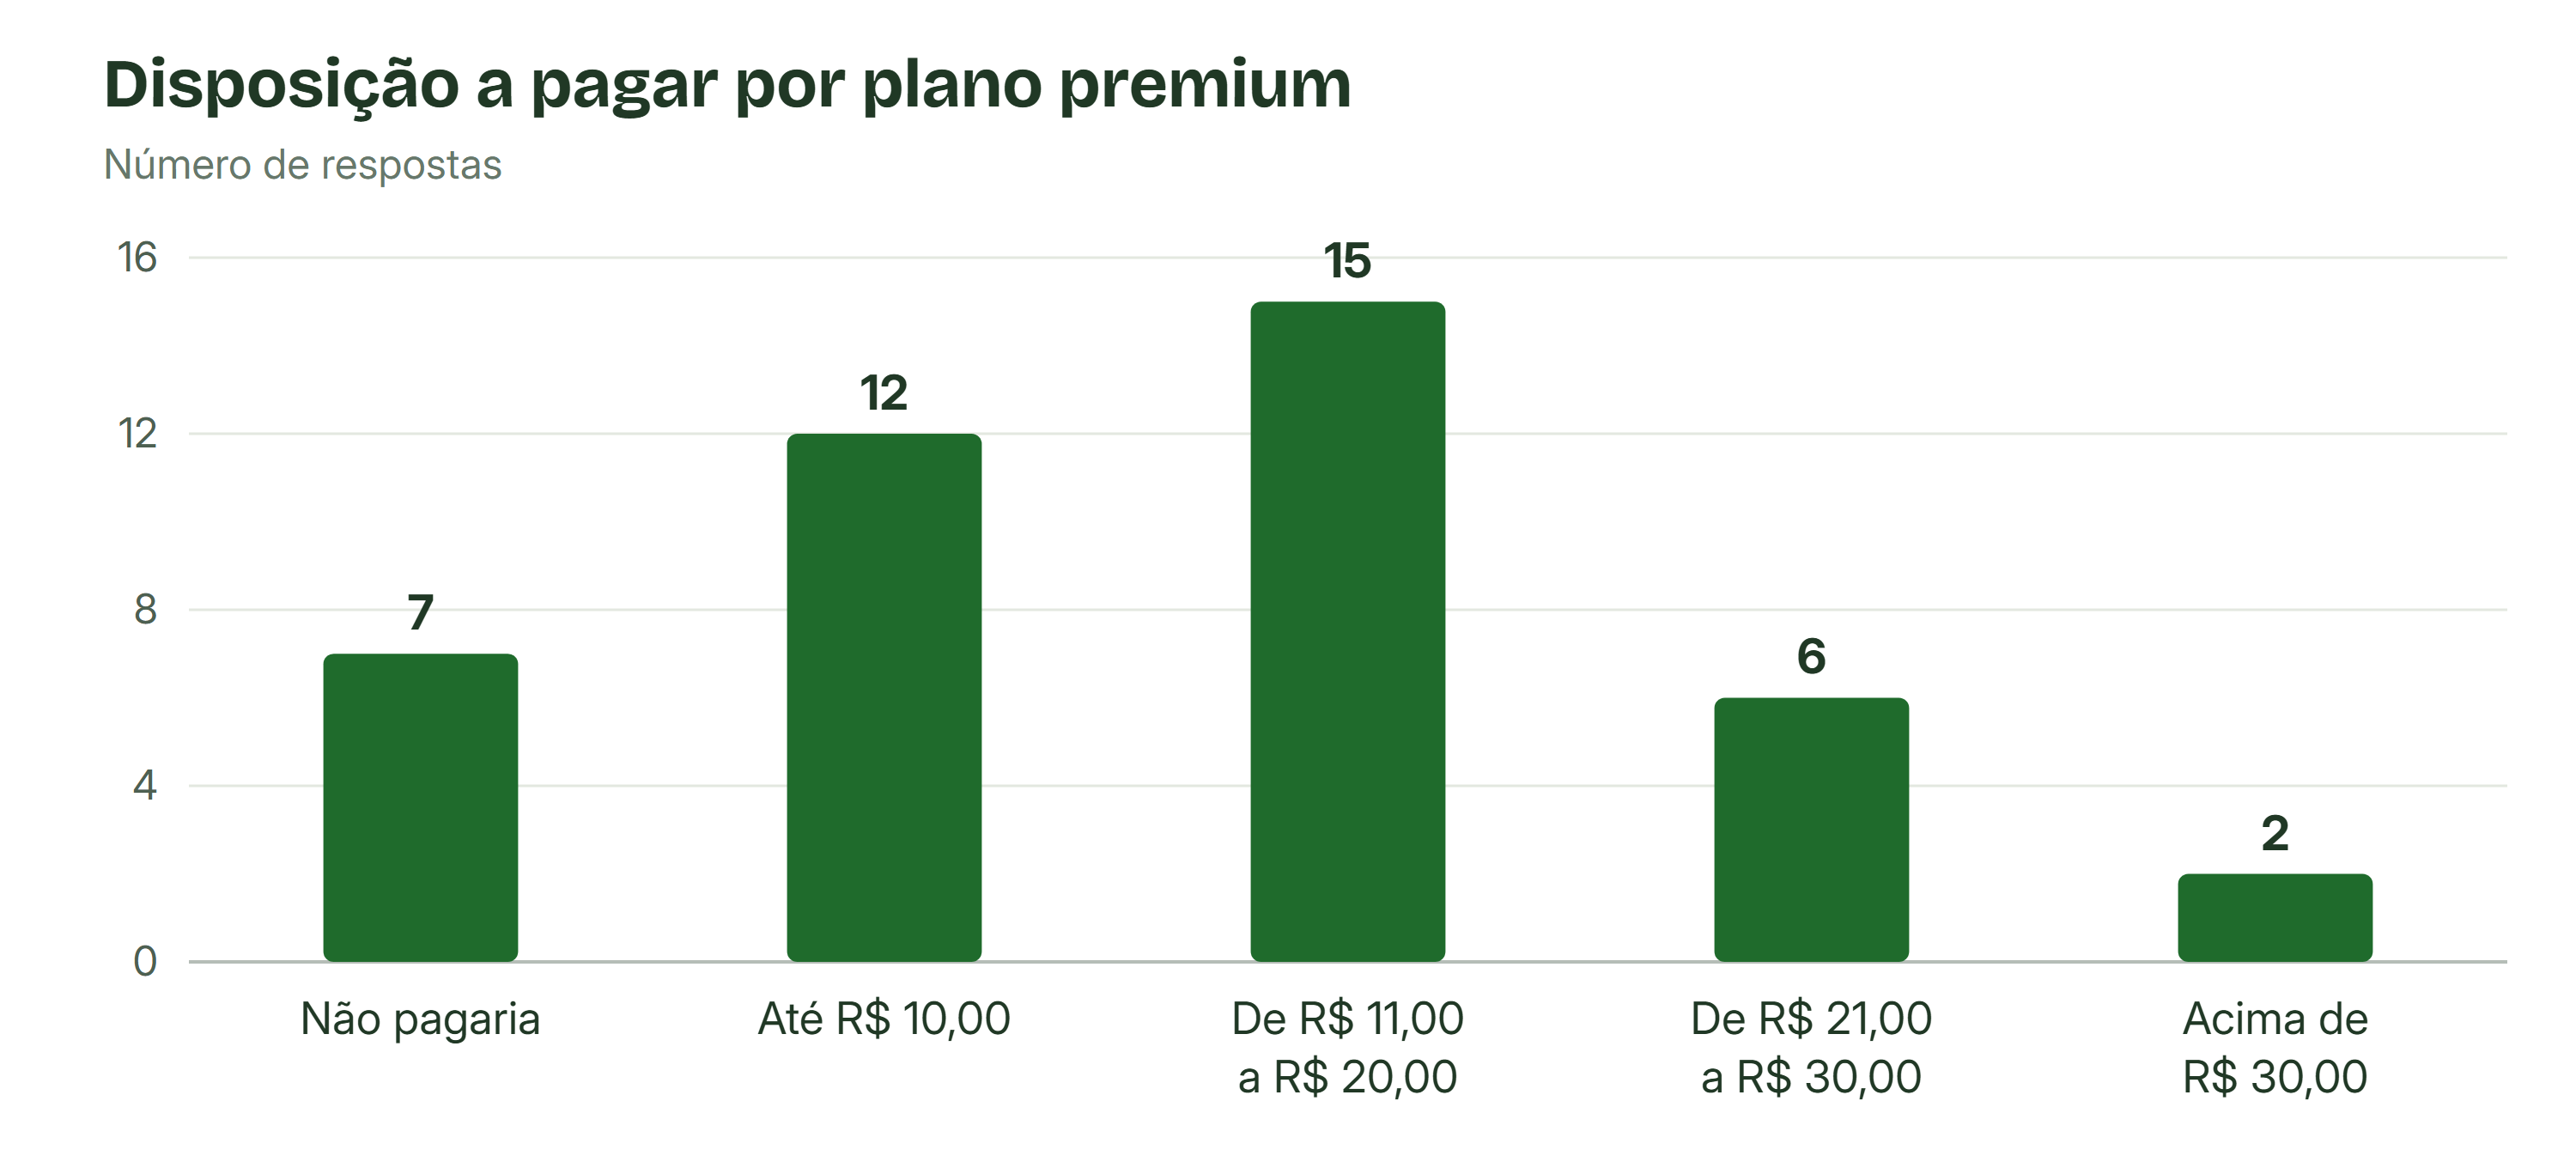
\includegraphics[width=0.8\textwidth]{images/pesquisa/pagarplano.png}
    \label{fig:pq_pagamento}
    \fontetabela{\textbf{Fonte:} Elaborado pelos autores (2026).}
\end{figure}

Portanto, ficou clara a demanda por uma solução que auxilie seus usuários na organização e compreensão das próprias finanças de forma conversacional, consolidando dados de múltiplas contas e entregando informações em linguagem natural por meio de um canal já amplamente adotado. Os dados coletados evidenciam que o problema é real, o canal é adequado e o interesse pelas funcionalidades propostas é concreto.

\section{Análise de viabilidade}

A viabilidade do projeto foi avaliada em duas perspectivas complementares: a operacional, considerando os custos de infraestrutura em diferentes estágios de crescimento, e a regulatória, considerando as exigências legais aplicáveis à solução.

Do ponto de vista operacional, a estratégia para o desenvolvimento e validação inicial do produto consiste em maximizar o uso de planos gratuitos (\textit{free tiers}) dos serviços de nuvem, consolidando todos os componentes da aplicação em um único servidor virtual privado (VPS). Essa abordagem viabiliza a execução do MVP (\textit{Minimum Viable Product}) com um custo estimado de aproximadamente R\$~780 a R\$~870 por mês, conforme detalhado no Quadro~\ref{quad:infra_dev}. Esse valor incorpora, além dos custos de infraestrutura em nuvem, a depreciação mensal dos equipamentos de desenvolvimento e as assinaturas de ferramentas de apoio à codificação com inteligência artificial. O único componente de infraestrutura com custo variável nessa fase são as chamadas às APIs de inteligência artificial da aplicação; os demais serviços — mensageria, cache, bancos de dados, integração com \textit{Open Finance} e \textit{WhatsApp Business} — operam dentro dos limites gratuitos suficientes para testes e validação com usuários reais.

{\small
\begin{longtable}{|p{3.5cm}|p{7.0cm}|p{3.0cm}|}
\caption{Infraestrutura estimada para a fase de desenvolvimento (MVP)} \label{quad:infra_dev} \\
\hline
\textbf{Componente} & \textbf{Especificação} & \textbf{Custo/mês} \\ \hline
\endfirsthead
\hline
\textbf{Componente} & \textbf{Especificação} & \textbf{Custo/mês} \\ \hline
\endhead
\hline
\multicolumn{3}{r}{\fontsize{10pt}{10pt}\selectfont\textit{Continua na próxima página}} \\
\endfoot
\hline
\multicolumn{3}{c}{\fontsize{10pt}{10pt}\selectfont \textbf{Fonte:} Elaborado pelos autores (2026).} \\
\endlastfoot
VPS principal & Hetzner CX22 (2 vCPU, 4 GB RAM, 40 GB SSD) — executa todos os microsserviços via Docker Compose & $\sim$R\$~30 \\ \hline
Message broker & Upstash Kafka (\textit{free tier}: 10.000 msgs/dia) & R\$~0 \\ \hline
Cache e sessões & Upstash Redis (\textit{free tier}: 10.000 comandos/dia, 256 MB) & R\$~0 \\ \hline
Banco relacional & PostgreSQL 16 \textit{self-hosted} no VPS via Docker & R\$~0 \\ \hline
Banco documental & MongoDB Atlas M0 (\textit{free tier}: 512 MB, criptografia em repouso inclusa) & R\$~0 \\ \hline
API de IA & OpenAI GPT-4o-mini (geração de respostas conversacionais) & $\sim$R\$~15--30 \\ \hline
API de embeddings & OpenAI text-embedding-3-small (vetorização para RAG) & $\sim$R\$~5--10 \\ \hline
WhatsApp Business & Meta Cloud API (1.000 conversas/mês gratuitas) & R\$~0 \\ \hline
Integração \textit{Open Finance} & Pluggy API (\textit{sandbox} gratuito para desenvolvimento) & R\$~0 \\ \hline
SSL e CDN & Let's Encrypt + Cloudflare (gratuitos) & R\$~0 \\ \hline
CI/CD & GitHub Actions (\textit{free tier}: 2.000 min/mês) & R\$~0 \\ \hline
Monitoramento & Grafana Cloud Free & R\$~0 \\ \hline
Backup & Cloudflare R2 (\textit{free tier}: 10 GB/mês) & R\$~0 \\ \hline
Equipamentos (depreciação) & 3 notebooks para desenvolvimento (vida útil 4 anos, valor médio R\$~5.000 cada) & $\sim$R\$~312 \\ \hline
IA para apoio a codificação & Claude Code (por desenvolvedor, 3 devs) & $\sim$R\$~330 \\ \hline
\textbf{Total estimado (MVP)} & & \textbf{$\sim$R\$~780--870} \\ \hline
\end{longtable}
}

À medida que o produto é validado e atinge escala de 10.000 usuários ativos, os \textit{free tiers} deixam de ser suficientes e a infraestrutura precisa ser dimensionada para suportar o volume de operações. Nesse cenário, estima-se uma média de 100.000 mensagens por dia, 40.000 sincronizações de transações e 100.000 chamadas às APIs de inteligência artificial. O Quadro~\ref{quad:infra_prod} apresenta os custos reais estimados para esse estágio, sem considerar planos gratuitos.

{\small
\begin{longtable}{|p{3.5cm}|p{7.0cm}|p{3.0cm}|}
\caption{Infraestrutura estimada para 10.000 usuários ativos (produção)} \label{quad:infra_prod} \\
\hline
\textbf{Componente} & \textbf{Especificação} & \textbf{Custo/mês} \\ \hline
\endfirsthead
\hline
\textbf{Componente} & \textbf{Especificação} & \textbf{Custo/mês} \\ \hline
\endhead
\hline
\multicolumn{3}{r}{\fontsize{10pt}{10pt}\selectfont\textit{Continua na próxima página}} \\
\endfoot
\hline
\multicolumn{3}{c}{\fontsize{10pt}{10pt}\selectfont \textbf{Fonte:} Elaborado pelos autores (2026).} \\
\endlastfoot
VPS (2 servidores) & Hetzner CX32 (4 vCPU, 8 GB RAM cada) via Docker Compose & $\sim$R\$~120 \\ \hline
Message broker & Upstash Kafka pay-as-you-go ($\sim$3M msgs/mês) & $\sim$R\$~50 \\ \hline
Cache e sessões & Redis \textit{self-hosted} no VPS & R\$~0 \\ \hline
Banco relacional & PostgreSQL 16 \textit{self-hosted} no VPS & R\$~0 \\ \hline
Banco documental & MongoDB Atlas M2 (2 GB RAM, 10 GB storage) & $\sim$R\$~150 \\ \hline
API de IA & OpenAI GPT-4o-mini ($\sim$100k chamadas/dia) & $\sim$R\$~800 \\ \hline
API de embeddings & OpenAI text-embedding-3-small & $\sim$R\$~50 \\ \hline
WhatsApp Business & Meta Cloud API ($\sim$50k conversas/mês) & $\sim$R\$~2.000 \\ \hline
Integração \textit{Open Finance} & Pluggy API (plano produção) & $\sim$R\$~500 \\ \hline
CI/CD e monitoramento & GitHub Actions + Grafana Cloud & $\sim$R\$~100 \\ \hline
Backup e CDN & Cloudflare R2 + Let's Encrypt & $\sim$R\$~30 \\ \hline
\textbf{Total estimado (produção)} & & \textbf{$\sim$R\$~3.800} \\ \hline
\end{longtable}
}

Com um custo operacional de aproximadamente R\$~3.800 mensais em produção, o ponto de equilíbrio (\textit{break-even}) é atingido com cerca de 166 assinantes do plano Pro (R\$~3.800 $\div$ R\$~22,90). Considerando uma taxa de conversão de 15\% de usuários gratuitos para o plano pago, isso corresponde a uma base total de aproximadamente 1.100 usuários cadastrados. A partir desse patamar, toda receita adicional representa margem de contribuição direta ao produto. Com 10.000 usuários e 15\% de conversão, a receita mensal recorrente seria de aproximadamente R\$~34.350, gerando uma margem operacional estimada de R\$~30.550 mensais.

\section{Preço de venda}\label{sec:preco}

A estratégia de monetização adotada é o modelo \textit{freemium}, no qual o usuário tem acesso inicial gratuito às funcionalidades essenciais e pode optar por um plano pago para obter recursos mais avançados. Essa abordagem reduz a barreira de entrada, facilita a experimentação e cria oportunidades de conversão à medida que o usuário percebe o valor da solução. O Quadro~\ref{quad:planos} detalha os planos disponíveis, suas funcionalidades e condições de faturamento.

{\small
\renewcommand{\arraystretch}{1.2}

\begin{longtable}{|p{5cm}|p{1.8cm}|p{2cm}|p{1.8cm}|p{2.7cm}|}
\caption{Planos e condições de faturamento da solução}
\label{quad:planos} \\
\hline
\textbf{Funcionalidades} &
\textbf{Plano} &
\textbf{Faturamento} &
\textbf{Desconto} &
\textbf{Valor mensal} \\ \hline
\endfirsthead

\hline
\textbf{Funcionalidades} &
\textbf{Plano} &
\textbf{Faturamento} &
\textbf{Desconto} &
\textbf{Valor mensal} \\ \hline
\endhead

\hline
\multicolumn{5}{r}{\textit{Continua na próxima página}} \\
\endfoot

\hline
\multicolumn{5}{c}{
\textbf{Fonte:} Elaborado pelos autores (2026).
} \\
\endlastfoot

Vinculação de 1 instituição via \textit{Open Finance};
consulta de saldo e extrato;
respostas conversacionais;
alertas básicos;
classificação de transações
&
Gratuito
&
---
&
---
&
R\$~0,00
\\ \hline

Acesso completo a todos os módulos:
instituições ilimitadas,
análises,
previsões,
metas,
resumos automáticos e
recomendações personalizadas
&
\multirow{2}{*}{Pro}
&
Mensal
&
---
&
R\$~22,90
\\ \cline{3-5}

&
&
Anual
&
$\sim$9\%
&
R\$~249,90/ano \newline
(R\$~20,83/mês)
\\ \hline

\end{longtable}
}